\documentclass[prl,twocolumn,amsmath,amssymb,superscriptaddress]{revtex4-2}

% You may use additional packages as you see fit
\usepackage{graphicx}
\usepackage{verbatim}
\usepackage{braket}
\usepackage{epsfig}
\usepackage{epstopdf}
\usepackage{amsfonts}
\usepackage{amsthm}
\usepackage{float}
\usepackage{amsmath}
\usepackage{amssymb}
\usepackage{color}
\usepackage[usenames,dvipsnames,svgnames,table]{xcolor}
\usepackage{dsfont}
\usepackage{color}
\usepackage{grffile}
\usepackage{bm}

% ones I added
\usepackage{hyperref}
\usepackage{multirow}
\hypersetup{colorlinks=true,linkcolor=NavyBlue,citecolor=BrickRed,urlcolor=NavyBlue}

%end of packages

\begin{document}

\title{Osmosis in Apple Flesh - SBI4UE Final Lab}
\author{Luyu W.V.K.}
\date{\today}

\begin{abstract}
    Enzyme and substrate concentration are variables that both influence the rate of enzymatic reactions. In this case, we investigate the relationship by changing the concentration of our enzyme (Catalase) and keeping our substrate concentration ($H_{2}O_2$) constant.
\end{abstract}
\maketitle

\section{Introduction}
Water potential difference is one of the key drivers of liquid movement along with kinematic pressure and surface tension forces.

Given a difference in the concentration of a solution inside and outside a barrier, there will be a driving force to equalize these concentrations.

This driving force is exhibited by movement of water in and out of the cell membrane in attempt to minimize the potential. This behavior is otherwise known as 'osmosis'.

This means that when the solution concentration within the cell is less than that outside, water will be pulled through the cell membrane. Conversely, when the solution concentration outside the cell is greater than inside, water will be excreted from the cell.

Because of this, we expect that when the solution inside and outside the cell are isotonic (of the same concentration), we will observe a negligible mass change.

\section{Methodology}
In this experiment we used transverse sections of Russett potatoes as our cell samples and sucrose ($C_{12}H_{22}O_{11}$) as our solute.

The solution was pre-diluted into 1.0M, 0.8M, 0.6M, 0.4M, 0.2M, and 0.0M solutions.

Potatoes were cut into 3cm, 2cm, and 1cm cylindrical slices. After massing them (precise to $\pm 0.01g$), we placed the potato slices into the sucrose solutions before leaving them to soak.

The soaking time was roughly 20 hours (varying by around $\pm 3$ hours between groups). This is adequate time for the full piece to equilibrize, according to literature results  (A. Lenart and J. M Flink, 1984) \cite{https://doi.org/10.1111/j.1365-2621.1984.tb00327.x}.

After soaking, potatoes were removed from the solution, lightly damped using paper towels to remove excess solution (qualitatively controlled). After being damped, they were immediately massed (once again accurate to $\pm 0.01g$).


\section{Results}

\begin{figure}[htb]
    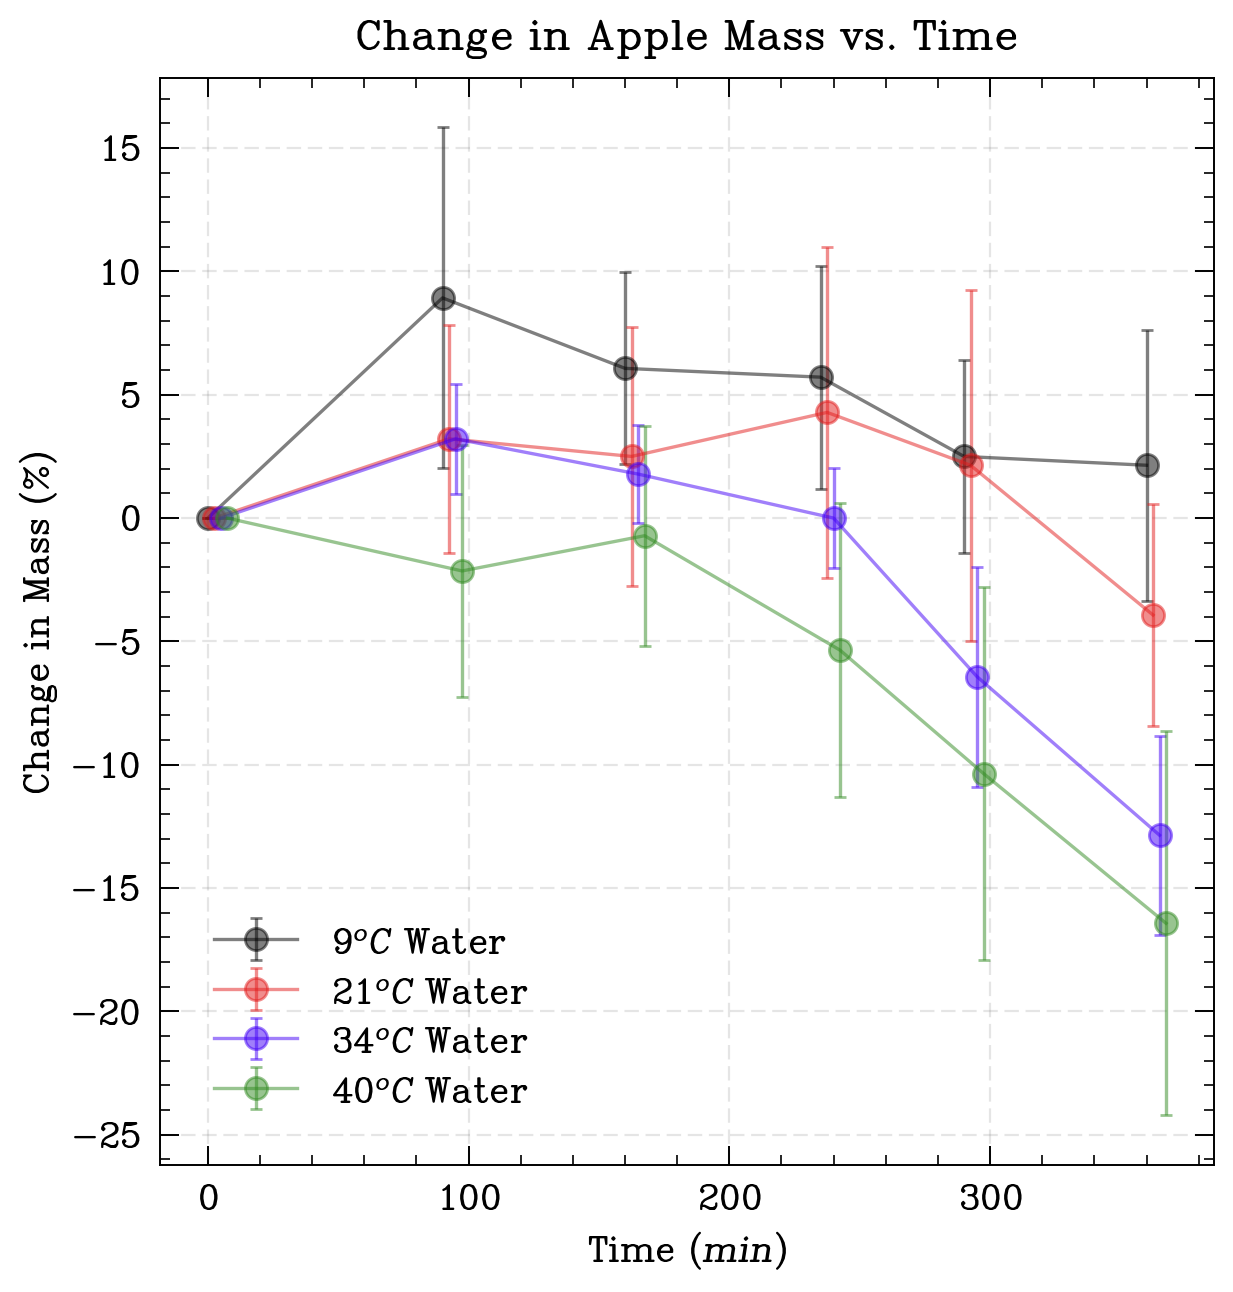
\includegraphics[width=1\linewidth]{change_in_mass.png}
    \caption{Percent mass change in apple in relation to time and temperature.}
    \label{fig:RelativeMassChange}
\end{figure}


\section{Errors}

\bibliography{refs}


\end{document}
